\chapter{Subjective validation of auralisation method}\label{chapter:test}

\section{Introduction}
In the previous chapter an overview was given of the auralisation tool. A
propagation model for aircraft sound was developed but still missing is an
emission model. An algorithm was presented for extracting select features from
recordings with the underlying idea of using those features for the development
of an empirical emission model.

The next step is to determine whether auralisations based on features obtained
from the described algorithm sound plausible. The purpose is to check not just
whether the auralisations sound like an aircraft, but also whether they sound
like the aircraft model and event that is being simulated. The assumption is
made that the propagation model represents the actual sound propagation
sufficiently good that inaccuracies in sound propagation are negligible and the
resulting differences are entirely due to the emission synthesis.

\subsubsection*{Perceptual validation}
The question is then how to validate the plausibility of the auralisations.
Comparing the overall and spectral sound pressure level as function of time
could be a first simple test to determine whether the signal power is approximately
correct. Signals with the same power may however still sound very different,
and how they sound may depend on a multitude of factors. Factors can be properties
of the sound, but also of the listener, or the environment.

Psychoacoustic measures describe how a sound is perceived by most listeners and
can therefore be used to characterise a sound. Many measures exist, but not all
measures are appliceable to all sounds and care should therefore be taken when
choosing measures. Examples of common measures are loudness, roughness and
sharpness. Instead of using measures, participants could be asked to rate
whether an auralisation sounds plausible. That would likely require a reference
sound, e.g. a recording.

Regardless of the method a variability exists in events that are considered
alike. For example, consider events that are all landingsm of a certain aircraft
type and with certain engines, and under meteorological conditions within a narrowly
defined range. In one event the pilot may vary the thrust differently than in
another event and that could already lead to audible differences.
Clearly, the variance across events should be accounted for.

\subsubsection*{Past work}
Several validations of auralisations have been done in the past. Maillard
conducted a quantitive and perceptual validation of road traffic auralisations
that were created using granular synthesis \cite{Maillard2014}. Pieren and
Heutschi conducted a small listening test to validate auralisations of
windturbines. Participants were presented with recordings and auralisations and
had to choose for each stimuli whether they thought it was a recording, an
auralisation, or whether they could not tell. Hoffmann combined a tyre-noise
prediction model with a car auralisation tool, and tested the perceptual
validity of the produced auralisations \cite{Hoffmann2016a,Hoffmann2016}. Tests
were done with semantic differentials using a categorical scale, and another
test done was a paired comparison test.

% \subsubsection*{Test methodologies}
A semantic differential is a set of semantic scales. Each scale is typically
defined by a bipolar combination of adjectives, e.g. \say{loud-silent}, and
divided into steps. A categorical scale is similar, however, instead of a
bipolar combination of adjectives with steps a single adjective is used with
steps. An example is \say{agree-disagree}, where each word is placed at opposite
ends of the scale. A paired comparison test is a type of test that can be used
to rank the items that are tested with respect to the attribute that is
investigated.

Another interesting type of test is MUSHRA, short for MUltiple Stimuli with
Hidden Reference and Anchor. The method is typically used to evaluate the
perceived quality of the output from lossy audio compression algorithms, but was
used by Southern to rate plausibility of auralisations of car pass-bys
\cite{Southern2016}.

\subsubsection*{Test overview}
This chapter describes a listening test that was conducted. The purpose of the
listening test was to check the plausiblity or perceptual validity of the
auralisations and a comparison was therefore made between recordings and
auralisations.

The hypothesis is that \emph{recordings and auralisations of aircraft of the same
type and under similar conditions are samples of the same group}.
Audible differences are likely to occur and are also acceptable, because even
among recordings of the same aircraft type there are audible differences.

Due to time-constraints psychoacoustic measures were not measured. Instead, an
overall similarity between stimuli was determined. Recordings were compared not
only with auralisations, but also with other recordings, and similarly,
auralisations with other auralisations. Each of these comparisons can be
considered a group. If the hypothesis is valid, then the distribution of the
group with comparisons between recordings and auralisations, should be the same
as the other two distributions.


\section{Method}

The goal of the listening test was to determine whether the auralisations sound
similar to the recordings they were based on. Participants were presented with
pairs of stimuli and asked to rate how similar they sounded.

Eight different sounds were considered and they were each 12 seconds long. The
sounds include the approach of an aircraft, its flyover and its distancing.
Because the character of the sounds varies considerably over time, they were
each split into parts of four seconds, corresponding to the approach, fly-over
and distancing. The listening test was also divided in these three parts. First,
participants were presented to all approach stimuli, then all fly-over stimuli
and finally all distancing stimuli. In each test part all stimuli combinations
were considered. Therefore, each part consisted of 28 pairs of stimuli of four
seconds.

Of the eight sounds four were recordings, and four were auralisations.
The recordings were randomly chosen from the sonAIR dataset. Each
auralisation was based on one of the recordings. Two aircraft types were
considered, an A320 and a RJ1H, as well as two events per aircraft type.
Fade in and fade out was applied to the stimuli. The signals were mono and
presented with headphones. Head-related transfer functions were not included.

Similarity is relative, and therefore an anchor is typically used. For each
part, participants were first given the set of stimuli, in order to become
familiar with the type of sounds and the spread in the sounds of that part, and
then continued with rating the pairs. The rating was done on an eleven point
Likert scale. The left side of the scale said ``not so much'' and the right side
``very much''. The scale was not numbered. The order of the stimuli was
randomised for each test and each part.

Figures \ref{fig:listening:results:recording-A320} and
\ref{fig:listening:results:simulation-A320} show spectrograms of some of the stimuli
that were used. The blade passing frequency and harmonics are not as prominent
in the auralisation as they are in the recording.

% \newpage
% \afterpage{
\begin{figure}[H]
  \centering
  \includegraphics[]{../figures/generated/listening/recording-A320}
  \caption{Spectrograms of the approach, fly-over and distancing parts of a recording of an A320.}
  \label{fig:listening:results:recording-A320}
% \end{figure}
%
% \begin{figure}
  \centering
  \includegraphics[]{../figures/generated/listening/turbulence-A320}
  \caption{Spectrograms of the approach, ``center`` and distancing parts of an auralisation of an A320.}
  \label{fig:listening:results:simulation-A320}
\end{figure}
% }
% \clearpage

\newpage
\section{Results}
The results of the participants were scaled linearly from 0 to 1 with 0
corresponding to ``not so much'' and 1 corresponding to ``very much''.
% Not all of the participants used the entire scale, and therefore they were rescaled per
% participant and per test part to use the full scale.
There were 17 participants, all graduate students, and of which the majority
studied acoustics. The results that are shown are obtained after joining the
data of all participants. % and all three test parts.
% Update raw results??
The listening test data can be found at \cite{Rietdijk2017a} and the
raw results along with a brief analysis at \cite{Rietdijk2017b}.

Table \ref{table:listening:results:analysis-parts} shows the mean $\mu$,
standard deviation $\sigma$ and amount of samples $n$ per group.
Averaging was done over participants. Table \ref{table:listening:results:analysis} is similar,
but now averaging was done not over only participants but also over the three test parts.

\begin{table}[H]
  \centering
  \caption{The mean value $\mu$, standard deviation $\sigma$ and amount of samples $n$ per aircraft type combination, and stimuli type combination. Averaging was done over participants and parts.}
  \label{table:listening:results:analysis}
  \input{../figures/generated/listening-analysis/table_analysis.tex}
\end{table}

Figure \ref{fig:listening:ratings-kde-overall} shows the distribution of the
similarity ratings grouped by aircraft and stimuli type combinations. The
vertical axes show kernel density estimations of how common the given ratings
were\footnote{ A kernel density estimation can be seen as a continuous version
of a histogram. Each sample is replaced by a kernel function centered at the
value of the sample. The curves are then summed to obtain a density and finally
normalised so that the area under the resulting curve is 1. }. A Gaussian kernel
was used. Averaging is done over participants and test parts.

Figures \ref{fig:listening:ratings-aircraft-type-combinations} and \ref{fig:listening:ratings-stimuli-type-combinations} show mostly the same curves as Figure \ref{fig:listening:ratings-kde-overall} but the curves are grouped.
Figure \ref{fig:listening:ratings-aircraft-type-combinations} shows the distribution of the similarity ratings grouped by
aircraft combination for both the recordings and the auralisations.
Figure \ref{fig:listening:ratings-stimuli-type-combinations} shows the distribution of the similarity ratings grouped by stimuli type combination
for both the A320 and the RJ1H. In both cases the results encompass all parts.

\begin{figure}[H]
  \centering
  \includegraphics{{{../figures/generated/listening-analysis/figure_kde}}}
  \caption{Similarity ratings grouped by both aircraft combinations and stimuli type combinations.}% Groups considering only recordings and compare only one aircraft type have relatively high similarity ratings. Groups that consider two aircraft types have relatively the lowest ratings. }
  \label{fig:listening:ratings-kde-overall}
\end{figure}

In Figures \ref{fig:listening:results:ratings-A320-parts} and
\ref{fig:listening:results:ratings-RJ1H-parts} the results were split by part.
To improve clarity, the amount of information is reduced by using Tukey boxplots.

Participants mentioned they noted larger differences at especially the approach of the events and the distancing.
A common answer to the question how many different aircraft they heard was ``two or three``.
Occasionally, the answer would start at ``two`` but go to ``two or more`` after they
were told they were listening to not only recordings but also simulations. Some
participants were surprised when told that simulations were included,
others said they had thought so, and a few of the participants were already
aware the test was possibly going to contain simulations.

\begin{table}[H]
  \centering
  \caption{The mean value $\mu$, standard deviation $\sigma$ and amount of samples $n$ per test part, aircraft type combination, and stimuli type combination. Averaging was done over participants.}
  \label{table:listening:results:analysis-parts}
  \input{../figures/generated/listening-analysis/table_analysis_parts.tex}
\end{table}


% \newpage
% \afterpage{
\begin{figure}
%     \centering
    \begin{subfigure}{0.5\textwidth}
        \includegraphics{{{../figures/generated/listening-analysis/figure1_ratings_recordings}}}
        \caption{Recordings}
        \label{fig:listening:ratings-aircraft-type-combinations:recordings}
    \end{subfigure}
    \begin{subfigure}{0.5\textwidth}
        \includegraphics{{{../figures/generated/listening-analysis/figure2_ratings_simulations}}}
        \caption{Auralisations}
        \label{fig:listening:ratings-aircraft-type-combinations:auralisations}
    \end{subfigure}
    \caption{Similarity ratings grouped by aircraft type combinations. The left figure shows the ratings for the recordings and the right figure for the auralisations.}
    \label{fig:listening:ratings-aircraft-type-combinations}
% \end{figure}
% \clearpage

% \begin{figure}
    \begin{subfigure}{0.5\textwidth}
        \includegraphics[]{{{../figures/generated/listening-analysis/figure3_ratings_A320}}}
        \caption{A320}
        \label{fig:listening:ratings-stimuli-type-combinations:A320}
    \end{subfigure}
    \begin{subfigure}{0.5\textwidth}
        \includegraphics[]{{{../figures/generated/listening-analysis/figure4_ratings_RJ1H}}}
        \caption{RJ1H}
        \label{fig:listening:ratings-stimuli-type-combinations:RJ1H}
    \end{subfigure}
    \caption{Similarity ratings grouped by stimuli type combinations. The left figure shows the ratings for the A320 and the right figure for the RJ1H.}
    \label{fig:listening:ratings-stimuli-type-combinations}
\end{figure}
% }
% \clearpage

% \begin{figure}[H]
%   \centering
%   \includegraphics[]{../figures/generated/listening-analysis/figure1_ratings_recordings}
%   \caption{Similarity ratings for the recordings grouped by aircraft type.}
%   \label{fig:ratings_recordings}
% \end{figure}
%
% \begin{figure}[H]
%   \centering
%   \includegraphics[]{../figures/generated/listening-analysis/figure2_ratings_simulations}
%   \caption{Similarity ratings for the auralisations grouped by aircraft type.}
%   \label{fig:ratings_simulations}
% \end{figure}
%
% \begin{figure}[H]
%   \centering
%   \includegraphics[]{../figures/generated/listening-analysis/figure3_ratings_A320}
%   \caption{Similarity ratings for the A320 grouped by stimuli type combinations.}
%   \label{fig:ratings_A320}
% \end{figure}
%
% \begin{figure}[H]
%   \centering
%   \includegraphics[]{../figures/generated/listening-analysis/figure4_ratings_RJ1H}
%   \caption{Similarity ratings for the RJ1H grouped by stimuli type combinations.}
%   \label{fig:ratings_RJ1H}
% \end{figure}


%
% \newpage
% \afterpage{
% \begin{float}
\begin{figure}[H]
  \centering
  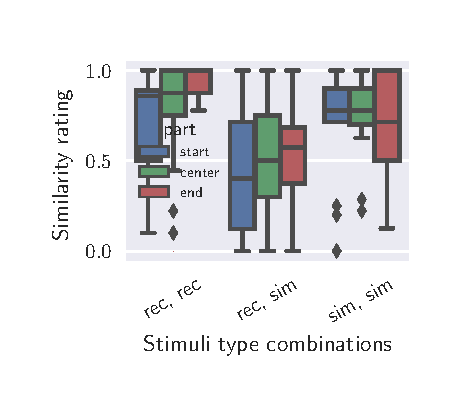
\includegraphics[]{../figures/generated/listening-analysis/figure5_ratings_part_A320}
  \caption{Similarity ratings for the A320 grouped by stimuli type combinations and stimuli part.}
  \label{fig:listening:results:ratings-A320-parts}
% \end{figure}
% TODO discuss

% \begin{figure}[H]
  \centering
  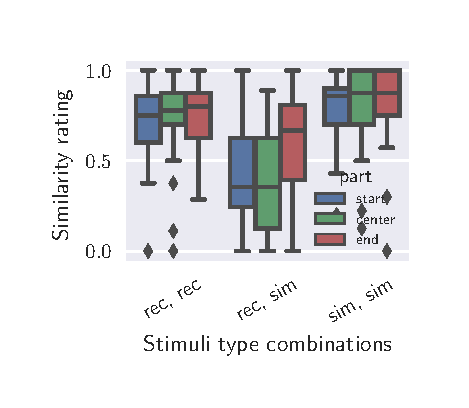
\includegraphics[]{../figures/generated/listening-analysis/figure6_ratings_part_RJ1H}
  \caption{Similarity ratings for the RJ1H grouped by stimuli type combinations and stimuli part.}
  \label{fig:listening:results:ratings-RJ1H-parts}
\end{figure}
% \end{float}
% TODO discuss
% }

\newpage
\section{Discussion}
Consider Tables \ref{table:listening:results:analysis} and
\ref{table:listening:results:analysis-parts}. The standard deviation of the
groups is mostly around 0.25, although a notable exception is the group in which
two recordings of A320's were compared. The standard deviation is only 0.09 and
the mean 0.89. Comparing that with the other groups, implies the two recordings
this group consists of are relatively closer to eachother than those in other
groups.
The highest mean values are achieved when comparing similar aircraft types,
regardless of whether the stimuli were recordings or auralisations. However,
when comparing a recording with an auralisation the mean value is lower. The
mean values of the groups comparing recordings and auralisations are
systematically below those of the groups comparing recordings or auralisations.
That would imply the hypothesis is not true.

Figure \ref{fig:listening:ratings-kde-overall} shows kernel density estimates of
the distributions of the nine groups. Some groups appear to follow a Gaussian
curve, however, not all. In certain cases there are also (close to) two maxima.
The similarity rating is a value given by participants after performing a
comparison of two items, and comparing them on whichever aspects they choose to
consider. Therefore, it is likely that the distributions are Gaussian. However,
because the ratings could only be given on a limited range this may skew the
distributions.

% Z-score and p-value?

As can be seen in Figure
\ref{fig:listening:ratings-aircraft-type-combinations:recordings}, the recordings of the A320's
are judged to be very similar to each other, and the recordings of the RJ1H's as quite similar to
each other as well. The A320's are not rated as very similar to the RJ1H's and therefore
it appears that the participants can discriminate between the two aircraft
types.
In the case of the auralisations, Figure
\ref{fig:listening:ratings-aircraft-type-combinations:auralisations}, the
results are similar in case of the A320's and the RJ1H's, although less convincing.
Furthermore, in this case the dissimilarity between the A320's and the RJ1H's isn't as large.
In fact, this distribution is relatively closer to the other two distributions than is the case with the recordings,
implying the auralisations, regardless of aircraft type, all sound more alike.

% participants can also discriminate between the aircraft types, but now the
% RJ1H's are judged to be relatively more similar than the A320's. Compared to the
% recordings the difference between the A320's and the RJ1H's is slightly smaller.

% One might argue from these findings that the whole set of auralisations is more similar than the set of recordings.

Another view on the data is presented in Figure
\ref{fig:listening:ratings-stimuli-type-combinations}. Were the hypothesis
valid, then the curves in each subfigure would have to overlap. While the
distributions of the groups that compare auralisations are quite similar to the
distributions comparing recordings, the groups comparing auralisations with
recordings are not similar at all. That would again imply the hypothesis is not
true and that the auralisations may appear to be different types of aircraft.

% The groups ``(rec, sim)'' contain pairs consisting of a recording and an auralisation, and the similarity ratings of these two groups are similar to the ``(A320, RJ1H)''
% groups in Figure \ref{fig:listening:ratings-aircraft-type-combinations}. Therefore,
% it would appear that listeners can discriminate between aircraft types, but that
% the auralisations are considered to be of different aircraft types than the
% recordings they are based on.

Figures \ref{fig:listening:results:ratings-A320-parts} and
\ref{fig:listening:results:ratings-RJ1H-parts} show the same data as \ref{fig:listening:ratings-stimuli-type-combinations}
but grouped further by stimuli part. Judging from Figure
\ref{fig:listening:results:ratings-A320-parts} there appears to be a
relative large dissimilarity between the approach and fly-over parts of the A320 recordings.
The distancing parts, however, are rated as very similar. The groups ``(rec,
rec)'' and ``(sim, sim)'' consist however of only 17 data points.

% When comparing auralisations
% and recordings there does not seem to be any especially good or bad part: the spread is relatively large and the mean is mediocre at
% and also between the ``end'' parts of the A320 auralisations.  each whereas
% the ``(rec, sim)'' group has 68 data points.

The participants mentioned relatively larger differences in the stimuli that
correspond to the approach of the aircraft (``start`` stimuli). During the
approach the tonal components are clearly audible compared to other parts of the
events due to the directivity. The feature-extraction algorithm was known to
underestimate the power and bandwidth of the blade passing frequency and its
harmonics because the algorithm was tuned for the Buzz-Saw tones. Therefore, a
likely explanation is that this underestimation of power and bandwidth is
causing audible differences between recordings and auralisations.
Furthermore, as described in section \ref{sec:tool:synthesis:synthesis}, an
incorrect distribution was used for the phase relation between the harmonics.

Finally, it should be noted that only two events per aircraft type were
considered. In a future test more events should be considered in order to
correctly represent the spread that exists in recordings of a certain aircraft
type.
